\documentclass[8pt]{article} % use larger type; default would be 10pt

%\usepackage[utf8]{inputenc} % set input encoding (not needed with XeLaTeX)
\usepackage{graphicx}
\usepackage{float}
\usepackage{subfig}
\usepackage{amsmath}
\usepackage{amsfonts}
\usepackage{hyperref}
\usepackage{harpoon}
\usepackage{enumitem}
\usepackage{multicol}
\usepackage[neverdecrease]{paralist}
\usepackage{enumerate}
\usepackage{cancel}
\usepackage{ulem}

\usepackage{mystyle}

\newcommand{\myexplain}[3]{#1\xrightarrow{\text{#2}}#3}
\newcommand{\myexplainf}[4]{#1\xrightarrow{\begin{subarray}{c}\text{#2}\\\text{#3}\end{subarray}}#4}
\newcommand{\myexplainfi}[5]{#1\xrightarrow{\begin{subarray}{c}\text{#2}\\\text{#3}\\\text{#4}\end{subarray}}#5}
\newcommand{\myfrac}[2]{^#1/_#2}

\title{Math 1540\\University Mathematics for Financial Studies\\2013-14 Term 1\\Suggested solutions for\\HW problems Sec. 2.1-2.2 (Linear Algebra)}
\begin{document}
\maketitle
\section{Section 2.1}
\begin{description}
	\newcommand{\mydet}[2]{\left|\begin{array}{#1}#2\end{array}\right|}
	\item[\# 3.]{{\it Evaluate the following determinants.\\\\}
	\begin{inparaenum}[(a)]
		\setcounter{enumi}{4}
		\item $\left|\begin{array}{rrr}1&3&2\\4&1&-2\\2&1&3\end{array}\right|$\qquad
		\setcounter{enumi}{6}
		\item $\left|\begin{array}{rrrr}2&0&0&1\\0&1&0&0\\1&6&2&0\\1&1&-2&3\end{array}\right|$
	  \end{inparaenum}\\\\
	We simply apply the recurrent formula for the determinant\\
	\begin{enumerate}[(a)]
		\setcounter{enumi}{4}
		\item\[\left|\begin{array}{rrr}1&3&2\\4&1&-2\\2&1&3\end{array}\right|=1\mydet{rr}{1&-2\\1&3}-3\mydet{rr}{4&-2\\2&3}
			+2\mydet{rr}{4&1\\2&1}=\]\[=1\cdot(1\cdot 3-1\cdot(-2))-3\cdot(4\cdot 3-2\cdot (-2))+2\cdot(4\cdot 1-2\cdot 1)=-39\]
		\setcounter{enumi}{6}
	\item Here we shall use expansion along the second row first, as it contains the biggest number of zeros
		\[\mydet{rrrr}{2&0&0&1\\0&1&0&0\\1&6&2&0\\1&1&-2&3}=1\cdot\mydet{rrr}{2&0&1\\1&2&0\\1&-2&3}=2\mydet{rr}{2&0\\-2&3}+1\cdot\mydet{rr}
		{1&2\\1&-2}=\]
		\[=2\cdot(2\cdot3-(-2)\cdot0)+1\cdot(1\cdot(-2)-1\cdot2)=8\]
	\end{enumerate}
	}
\item[\# 4.]{{\it Evaluate the following determinants by inspection.\\\\}
	\begin{inparaenum}[(a)]
		\setcounter{enumi}{1}
		\item $\mydet{rrr}{2&0&0\\4&1&0\\7&3&-2}$\qquad
		\item $\mydet{rrr}{3&0&0\\2&1&1\\1&2&2}$\qquad
		\item $\mydet{rrrr}{4&0&2&1\\5&0&4&2\\2&0&3&4\\1&0&2&3}$
	  \end{inparaenum}\\\\
	  \begin{enumerate}[(a)]
		  \item As the matrix is lower triangular, determinant is equal to the product of the elements on a diagonal
			  \[\mydet{rrr}{2&0&0\\4&1&0\\7&3&-2}=2\cdot1\cdot(-2)=-4\]
			  \item First we may apply the recurrent formula along the first row. This can be done by inspection, as first row has
				  only one nonzero element
				  \[\mydet{rrr}{3&0&0\\2&1&1\\1&2&2}=3\cdot\mydet{rr}{1&1\\2&2}\]
				  Now the $2\times2$ determinant is zero, as two rows of the matrix are proportional, hence it is singular. 
				  Thus
				  \[\mydet{rrr}{3&0&0\\2&1&1\\1&2&2}=3\cdot\mydet{rr}{1&1\\2&2}=0\]
			  \item The determinant is zero, as matrix contains zero column, hence is singular
				  \[\mydet{rrrr}{4&0&2&1\\5&0&4&2\\2&0&3&4\\1&0&2&3}=0\]
	  \end{enumerate}
	}
\item[\# 6.]{{\it Find all the values of $\lambda$ for which the following determinant will equal 0.}
	\[\mydet{cc}{2-\lambda&4\\3&3-\lambda}\]
	First we write the determinant of above $2\times2$ matrix
	\[\mydet{cc}{2-\lambda&4\\3&3-\lambda}=(2-\lambda)\cdot(3-\lambda)-3\cdot4=\lambda^2-5\lambda-6\]
	As we want this quantity to be zero, we end up with solving quadratic equation. The solutions are $\lambda=-1$ and $\lambda=6$.
	}
\item[\# 10.]{{\it Use mathematical induction to prove that if $A$ is an $(n+1)\times(n+1)$ matrix with two identical rows, then $\det(A)=0$.}
	We shall use the induction on the $n$ in the statement. Base case is $n=1$. In this case the statement can be verified directly
	\[\mydet{cc}{a&b\\a&b}=ab-ab=0\]
	Now, let us assume that it is correct for some $n\geq 1$ and try to show that it will also hold for $n+1$ then. For this purpose, let
	$A$ be $(n+2)\times(n+2)$ matrix with rows, say $\mathbf{v_1},\mathbf{v_2},\dots,\mathbf{v_{n+2}}$, of which two, say $\mathbf{v_i}$
	and $\mathbf{v_j}$ are equal. Now, applying recurrent formula along any row, $\mathbf{v_k}=(v_k^1,v_k^2,\dots,v_k^{n+2})$,
	such that $k\neq i$ and $k\neq j$ (which is possible as $n+2\geq 3$, we get
	\[\myabs{A}=v_k^1\cdot\myabs{A_1}-v_k^2\myabs{A_2}\pm\dots+(-1)^{n+1}\cdot v_k^{n+2}\myabs{A_{n+2}}\]
	where $A_l$ is matrix $A$ with $k$-th row and $l$-th column removed for $1\leq l\leq n+2$. Now, for any $A_l$ it will still contain two 
	identical rows, as each of $\mathbf{v_i}$ and $\mathbf{v_j}$ will still be present, although cut by one element (corresponding to $l$-th
	column removed). Hence, by inductive assumption, $\myabs{A_1}=\myabs{A_2}=\dots=\myabs{A_{n+2}}=0$ and therefore
	\[\myabs{A}=v_k^1\cdot\myabs{A_1}-v_k^2\myabs{A_2}\pm\dots+(-1)^{n+1}\cdot v_k^{n+2}\myabs{A_{n+2}}=0\]
	which justifies inductive step and finishes the proof.
	}
\item[\# 11.]{{\it Let $A$ and $B$ be $2\times2$ matrices.}
	\begin{enumerate}[(a)]
		\item{\it Does $\det(A+B)=\det(A)+\det(B)$?}
		\item{\it Does $\det(AB)=\det(A)\det(B)$?}
		\item{\it Does $\det(AB)=\det(BA)$?}
	\end{enumerate}
	\begin{enumerate}[(a)]
		\item Sometimes, yes, e.g.
			\[\mydet{rr}{0&0\\0&2}=\mydet{rr}{1&0\\0&1}+\mydet{rr}{-1&0\\0&1}\]
			and sometimes, no
			\[4=\mydet{rr}{2&0\\0&2}\neq\mydet{rr}{1&0\\0&1}+\mydet{rr}{1&0\\0&1}=2\]
			Some less trivial examples of when $\det(A+B)=\det(A)+\det(B)$ may hold, see the solution of Problem 12 below.
		\item{
			\newcommand{\uuuline}[1]{\dashuline{#1}}
			\newcommand{\uuuuline}[1]{\dotuline{#1}}
			Yes. This can be verified easily just by writing down the explicit formulae
			\[\mydet{rr}{a&b\\c&d}\cdot\mydet{rr}{a'&b'\\c'&d'}=(ad-bc)(a'd'-b'c')=\underline{ada'd'}
			-\underline{\underline{adb'c'}}-\uuuline{bca'd'}+\uuuuline{bcb'c'}=\]
			\[=\cancel{aa'cb'}+\underline{aa'dd'}
			+\uuuuline{bc'cb'}+\xcancel{bc'dd'}-\cancel{ca'ab'}-\uuuline{ca'bd'}-\underline{\underline{dc'ab'}}-\xcancel{dc'bd'}=\]
			\[=\mydet{cc}{aa'+bc'&ab'+bd'\\ca'+dc'&cb'+dd'}
			=\det\mybra{\begin{bmatrix}a&b\\c&d\end{bmatrix}\cdot\begin{bmatrix}a'&b'\\c'&d'\end{bmatrix}}\]
				}
		\item Yes and this is an implication of what we have proven in a previous item, as
			\[\det(AB)=\det(A)\det(B)=\det(B)\det(A)=\det(BA)\]
	\end{enumerate}
	}
\item[\# 12.]{{\it Let $A$ and $B$ be $2\times2$ matrices and let}
	\[C=\begin{pmatrix}a_{11}&a_{12}\\b_{21}&b_{22}
	\end{pmatrix},\quad D=\begin{pmatrix}b_{11}&b_{12}\\a_{21}&a_{22}\end{pmatrix},\quad E=\begin{pmatrix}0&\alpha\\\beta&0\end{pmatrix}\]
	\begin{enumerate}[(a)]
		\item{\it Show that $\det(A+B)=\det(A)+\det(B)+\det(C)+\det(D)$.}
		\item{\it Show that if $B=EA$ then $\det(A+B)=\det(A)+\det(B)$.}
	\end{enumerate}
	\begin{enumerate}[(a)]
		\item{
			This is easy, as
			\[\det(A+B)=\begin{vmatrix}a_{11}+b_{11}&a_{12}+b_{12}\\a_{21}+b_{21}&a_{22}+b_{22}\end{vmatrix}=\]
				\[=\underline{a_{11}a_{22}}+\underline{\underline{a_{11}b_{22}}}+\dashuline{b_{11}a_{22}}+
				\dashuline{\dashuline{b_{11}b_{22}}}-\dotuline{a_{21}a_{12}}-\dotuline{\dotuline{a_{21}b_{12}}}
				-\uwave{b_{21}a_{12}}-\uwave{\uwave{b_{21}b_{12}}}=\]
				\[=(\uline{a_{11}a_{22}}-\dotuline{a_{12}a_{21}})+(\dashuline{\dashuline{b_{11}b_{22}}}-
				\uwave{\uwave{b_{12}b_{21}}})+(\uuline{a_{11}b_{22}}-\dotuline{a_{12}b_{21}})+(\dashuline{
				\dashuline{b_{11}a_{22}}}-\dotuline{\dotuline{a_{21}b_{12}}})=\]
				\[=\begin{vmatrix}a_{11}&a_{12}\\a_{21}&a_{22}\end{vmatrix}+\begin{vmatrix}b_{11}&b_{12}\\b_{21}&b_{22}
				\end{vmatrix}+\begin{vmatrix}a_{11}&a_{12}\\b_{21}&b_{22}
				\end{vmatrix}+\begin{vmatrix}b_{11}&b_{12}\\a_{21}&a_{22}\end{vmatrix}=\det(A)+\det(B)+\det(C)+\det(D)\]
				}
		\item{To see that $\det(A+B)=\det(A)+\det(B)$ when $B=EA$, note that in this case 
			\[\begin{vmatrix}b_{11}&b_{12}\\b_{21}&b_{22}\end{vmatrix}=
			B=EA=\begin{vmatrix}0&\alpha\\\beta&0\end{vmatrix}\cdot\begin{vmatrix}a_{11}&a_{12}\\a_{21}&a_{22}\end{vmatrix}=
				\begin{vmatrix}\alpha\cdot a_{21}&\alpha\cdot a_{22}\\\beta\cdot a_{11}&\beta\cdot a_{12}\end{vmatrix}\]
			hence
			\[C=\begin{vmatrix}a_{11}&a_{12}\\b_{21}&b_{22}\end{vmatrix}=\begin{vmatrix}a_{11}&a_{12}\\\beta\cdot a_{11}&
				\beta\cdot a_{12}\end{vmatrix}\implies\det(C)=0\]
				\[D=\begin{vmatrix}b_{11}&b_{12}\\a_{21}&a_{22}\end{vmatrix}=\begin{vmatrix}\alpha\cdot a_{21}&
					\alpha\cdot a_{22}\\a_{21}&a_{22}\end{vmatrix}\implies\det(D)=0\]
			As both $D$ and $C$ have two rows being identical, thus their determinant is zero by the conclusion of Problem
			10. Therefore, the conclusion of a previous subproblem gives us
			\[\det(A+B)=\det(A)+\det(B)+\det(C)+\det(D)=\det(A)+\det(B)\]
			}
	\end{enumerate}
	}
\item[\# 13.]{{\it Let $A$ by symmetric tridiagonal matrix (i.e., $A$ is symmetric and $a_{ij}=0$ whenever $\myabs{i-j}>1$). Let $B$ be the matrix
	formed from $A$ by deleting the first two rows and columns. Show that \[\det(A)=a_{11}\det(M_{11})-a_{12}^2\det(B)\]}
	Simply applying the recurrent formula for determinant along the first row we get	
	\[\det(A)=\begin{vmatrix}
		a_{11}&a_{12}&0&0&\dots&0\\
		a_{12}&a_{22}&a_{23}&0&\dots&0\\
		0&a_{23}&a_{33}&a_{34}&\dots&0\\
		0&0&a_{34}&a_{44}&\dots&0\\
		\vdots&\vdots&\vdots&\vdots&\ddots&\vdots\\
		0&0&0&0&\dots&a_{nn}
	\end{vmatrix}=
		a_{11}\det(M_{11})-a_{12}\begin{vmatrix}
		a_{12}&a_{23}&0&\dots&0\\
		0&a_{23}&a_{34}&\dots&0\\
		0&a_{34}&a_{44}&\dots&0\\
		\vdots&\vdots&\vdots&\ddots&\vdots\\
		0&0&0&\dots&a_{nn}
			\end{vmatrix}\]
			Applying expansion along the first column to the second determinant, we further get
			\[\det(A)=
		a_{11}\det(M_{11})-a_{12}\begin{vmatrix}
		a_{12}&a_{23}&0&\dots&0\\
		0&a_{23}&a_{34}&\dots&0\\
		0&a_{34}&a_{44}&\dots&0\\
		\vdots&\vdots&\vdots&\ddots&\vdots\\
		0&0&0&\dots&a_{nn}
			\end{vmatrix}=\]\[=
			a_{11}\det(M_{11})-a_{12}^2\begin{vmatrix}
				a_{23}&a_{34}&\dots&0\\
				a_{34}&a_{44}&\dots&0\\
				\vdots&\vdots&\ddots&\vdots\\
				0&0&\dots&a_{nn}
			\end{vmatrix}=\]\[=a_{11}\det(M_{11})-a_{12}^2\det(B)\]
	}
%Sec 2.1 #3eg, 4bcd, 6, 10, 11, 12, 13
\section{Section 2.2}
\item[\# 4.]{{\it Find all possible choices of $c$ that would make the following matrix singular
	\[\begin{pmatrix}1&1&1\\1&9&c\\1&c&3\end{pmatrix}\]}
	Again, it is easy to write down the determinant explicitly in this case. We shall use this example to introduce the so-called {\it Rule
	of Sarrus} (see, for example \url{http://en.wikipedia.org/wiki/Rule_of_Sarrus}), which is a way to memorize the formula for the determinant
	of a $3\times3$ matrix. It is the most easily understood when looking on a picture below.
	\begin{figure}[H]
	\centering
	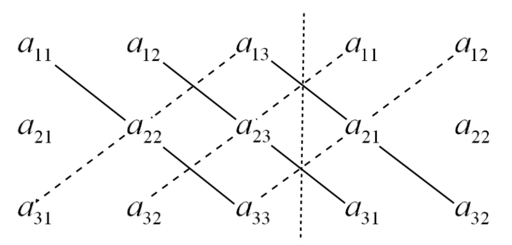
\includegraphics[width=0.6\textwidth]{sarrus_rule.png}
	\end{figure}
	Given the matrix $A$ with entries $(a_{ij})_{i,j=1}^3$ we essentially write out the first 2 columns of the matrix to the right of the
	3rd column. Then we add the product products of the diagonals going from top to bottom (solid on an illustration above)
	and subtract the products of the diagonals going from bottom to top (dashed). In our case this yields
	\[\begin{pmatrix}1&1&1\\1&9&c\\1&c&3\end{pmatrix}=1\cdot9\cdot3+1\cdot c\cdot 1+1\cdot 1\cdot c-1\cdot 9\cdot1-1\cdot c\cdot c-1\cdot1\cdot
		3=15+2c-c^2\]
		As we are interested in the values of $c$, that make the determinant vanish, we are end up with solving quadratic equation
		$15+2c-c^2=0$ and its solutions are $c=-3$ and $c=5$.
		}
\item[\# 5.]{{\it Let $A$ be an $n\times n$ matrix and $\alpha$ a scalar. Show that \[\det(\alpha A)=\alpha^n\det(A)\]}
	Let us define by $E_i(\alpha)$ the identity matrix with $i$-th row multiplied by $\alpha$. Note that $E_i(\alpha)$ is an elementary
	matrix (hence $\det(E_i(\alpha)A)=\det(E_i(\alpha))\det(A)=\alpha\det(A)$) 
	and multiplications on the left by $E_i(\alpha)$ corresponds to multiplication of the $i$-th row by $\alpha$, hence $\alpha A=E_1(\alpha)
	E_2(\alpha)\cdot\hdots\cdot E_n(\alpha)$. Therefore, 
	\[\det(\alpha A)=\det(E_1(\alpha))\det(E_2(\alpha))\cdot\hdots\cdot\det(E_n(\alpha))\det(A)=\alpha^n\det(A)\]
	}

\end{description}
%Sec 2.2 #4, 5
\end{document}
